\singlespacing

\mychapter{myblue}{Discussion}
  \sectionblue*{Résumé}
    \begin{center}
      \begin{tabular}{c}
        \fcolorbox{mydarkblue}{mylightblue}{
        \begin{minipage}[][4cm][c]{0.8\linewidth}
          \sffamily
          Nous détaillerons ici notre méthode d'Intégration Transcriptome Interactome. J'ai choisi d'inclure dans cette section nos chapitres. Ces chapitres étant trop long, ils se trouvent dans les Annexes \ref{app:Garcia2011} \ref{app:Garcia2013}. Je donnerai également une brève description des outils utilisés, ainsi qu'une description en détail de l'algorithme ITI\index{ITI}.
        \end{minipage}}\\
        \\[2ex]
        \begin{minipage}[][4cm][c]{0.9\linewidth}
          \mtcsetdepth{minitoc}{1}
          \minitoc
        \end{minipage}
      \end{tabular}
    \end{center}
    \newpage

\doublespacing

  \section{\textcolor{myblue}{Importance des données initiales}}
      Le jeu de données d'apprentissage a une grande importance lors de l'établissement d'une signature prédictive \citep{Michiels2005}.


    \subsection{\textcolor{myblue}{Effet de la variation des jeux de données d'entraînement}}
      Les validations croisées réalisées lors des analyses supervisée et non-supervisée nous ont permis de comparer l'apport des différents jeux de données, et notamment de vérifier -> effet labo, effet plateforme...
    \subsection{\textcolor{myblue}{Effet de la variation de la nature des interactomes}}
      Test sur in silico + complexes

  \section{\textcolor{myblue}{Caractéristique des signatures réalisées}}

    Nous avons récupéré les listes des sondes constituants les signatures (70g (vVijver), 76g (Wang), 97g (GGI)). Nous avons utilisé les annotations les plus récentes des sondes, avons enlevé les doublons, et n'avons pas considéré les EST. Les annotations des sondes ayant changé, il peut y avoir une variation sur le nombre de gènes, c'est pourquoi nous trouvons un seul gène commun entre les signatures de vVijver et Wang alors que Chuang en trouvait 3. C'est également la raison pour laquelle la signature GGI que nous avons réalisé contient 108 gènes (et non 97 comme précisé dans la littérature).

    \begin{figure}
      \begin{center}
        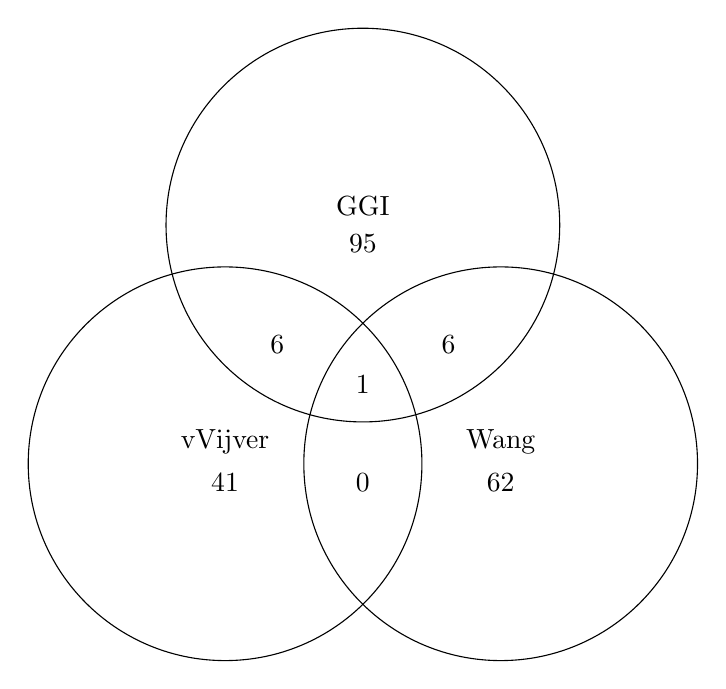
\begin{tikzpicture}
          \tikzset{venn circle/.style={draw,circle,minimum width=5cm}}
          \node [venn circle] (A) at (0,0){};
            \node [above] at (A) {vVijver};
            \node [below] at (A) {41};
          \node [venn circle] (B) at (60:3.5cm){};
            \node [above] at (B) {GGI};
            \node [below] at (B) {95};
          \node [venn circle] (C) at (0:3.5cm){};
            \node [above] at (C) {Wang};
            \node [below] at (C) {62};
          \node[left]  at (barycentric cs:A=1/2,B=1/2)      {6};
          \node[below] at (barycentric cs:A=1/2,C=1/2)      {0};
          \node[right] at (barycentric cs:B=1/2,C=1/2)      {6};
          \node at (barycentric cs:A=1/3,B=1/3,C=1/3){1};
        \end{tikzpicture}
      \end{center}
      \caption{Diagramme de Venn montrant les gènes communs entre les différentes signatures classiques.}
    \end{figure}

    \subsection{\textcolor{myblue}{Stabilité}}
      Plus stable  -> performances similaires quelque que soit les jeux de données d'entraînement
    \subsection{\textcolor{myblue}{Robustesse}}
      Plus robuste -> performances 
    \subsection{\textcolor{myblue}{Reproductibilité}}

    \subsection{\textcolor{myblue}{Significativité}}
      \citep{Fan2006}
      \citep{Haibe-Kains2008}

    \subsection{\textcolor{myblue}{Taille des sous-réseaux}}
    La question biologique posée a son importance.
    Par exemple, si c'est la différentiation entre deux types de cancer où beaucoup de gènes sont différentiellement exprimés, comme pour la leucémie myéloïde aiguë et la leucémie lymphoblastique aiguë, peu de gènes peuvent suffire pour différencier les deux conditions cliniques \citep{Dobbin2008}.

    Dans le cas de la question de pronostic, les différences d'expression entre gènes sont moins évidentes.

    C'est pourquoi les sous-réseaux ont une taille plus importante.

  \section{\textcolor{myblue}{Conclusion}}
  